\chapter{Reconstruction of Top Kinematics}

As presented in previous chapter, the $t\bar{t}$ dileptonic final state does not have a complete reconstruction 
of the final state. Two neutrinos are not detected and only their transverse energy can be measured. Thus additional
assumptions are needed to define the full final state kinematics of the $t\bar{t}$ decay products.

This section describes a method used for the kinematic reconstruction of $t\bar{t}$ in the dilepton final state. A mathematical
background as well as a performance description of the method are revealed.

\section{Mathematical Background}\label{sec:MatBg}

The problem of two not fully reconstructed neutrinos can be solved by setting certain constrains:

\begin{itemize}
 \item \textit{t and $\bar{t}$ masses} are assumed to be equal and constrained to the same value of 172.5 GeV\cite{PDG-2012};
 \item The whole missing transverse energy $E_{T}^{miss}$ of the event is assumed to arise entirely
 from the two neutrinos from the $t\bar{t}$ decay;
 \item \textit{The $W^{\pm}$ masses} are assumed to be equal and constrained to the value which is randomly taken
 from the generator $W^{\pm}$ mass spectrum.
\end{itemize}

These assumptions lead to the system of six equations with six unknowns (three momentum components of two neutrinos).
The equations are written down assuming the CMS coordinate system (see sec. \ref{sec:CMS}):

\begin{align}\label{alg:LS1}
 E^{miss}_{T_{x}} & =  p_{\nu_{x}} + p_{\bar{\nu}_{x}} \\
 %
 E^{miss}_{T_{y}} & =  p_{\nu_{y}} + p_{\bar{\nu}_{y}} \\
 %
 m^{2}_{W^{+}} & = (E_{l^{+}} + E_{\nu})^{2} - (p_{l^{+}_{x}} + p_{\nu_{x}})^{2} - (p_{l^{+}_{y}} + p_{\nu_{y}})^{2} - (p_{l^{+}_{z}} + p_{\nu_{z}})^2 \\
 %
 m^{2}_{W^{-}} & = (E_{l^{-}} + E_{\bar{\nu}})^{2} - (p_{l^{-}_{x}} + p_{\bar{\nu}_{x}})^{2} - (p_{l^{-}_{y}} + p_{\bar{\nu}_{y}})^{2} - (p_{l^{-}_{z}} + p_{\bar{\nu}_{z}})^2 \\
 % 
 m_{t}^{2} & = (E_{b} + E_{l^{+}} + E_{\nu})^{2} - (p_{b_{x}} + p_{l^{+}_{x}} + p_{\nu_{x}})^2 \nonumber \\
           & - (p_{b_{y}} + p_{l^{+}_{y}} + p_{\nu_{y}})^2 - (p_{b_{z}} + p_{l^{+}_{z}} + p_{\nu_{z}})^2 \\
 %
 m_{\bar{t}}^{2} & = (E_{\bar{b}} + E_{l^{-}} + E_{\bar{\nu}})^{2} - (p_{\bar{b}_{x}} + p_{l^{-}_{x}} + p_{\bar{\nu}_{x}})^2 \nonumber \\
                 & - (p_{\bar{b}_{y}} + p_{l^{-}_{y}} + p_{\bar{\nu}_{y}})^2 - (p_{\bar{b}_{z}} + p_{l^{-}_{z}} + p_{\bar{\nu}_{z}})^2\label{alg:LS6} 
\end{align}

Here the the $E_{l^{\pm}}$ and $p_{l^{\pm}_{x,y,z}}$ correspond to the lepton(antilepton) energy and momentum components respectively; 
$E_{b/\bar{b}}$ and $p_{b/\bar{b}_{x,y,z}}$ are the $b$/$\bar{b}$-jet energy and momentum components respectively; the $E^{miss}_{T_{x,y}}$ are
the two components of the missing transverse energy.
These are the characteristics of the reconstructed objects from the detector information directly, as described in the chapter \ref{chapt:event_selection}.
The six unknowns are the neutrino momentum components $p_{\nu/\bar{\nu}_{x,y,z}}$ and the neutrino energies are just composed from momenta:

\begin{equation}
 E_{\nu/\bar{\nu}}^{2} = p_{\nu/\bar{\nu}_{x}}^{2} + p_{\nu/\bar{\nu}_{y}}^{2} + p_{\nu/\bar{\nu}_{z}}^{2}
\end{equation}

The analytical solution of the system of equations (\ref{alg:LS1}--\ref{alg:LS6}) was proposed in \cite{LSpaper}. After a number of transformations
the system is reduced to one equation:

\begin{equation}\label{eq:eqLSf}
 0 = h_{0} p_{\nu_{x}}^{4} + h_{1} p_{\nu_{x}}^{3} + h_{2} p_{\nu_{x}}^{2} + h_{3} p_{\nu_{x}} + h_{4},
\end{equation}

where the coefficients $h_{0} -- h_{4}$ are described in \cite{LSpaper, LSerrat}. They depend on the four-momenta of the reconstructed 
leptons and jets and also on the missing transverse energy $E_{T}^{miss}$. 

The equation \ref{eq:eqLSf} is a fourth order polynomial. In the ideal case after solving it as described in \cite{LSpaper} one gets
in 80$\%$ of the cases two solutions and in 20$\%$ of the cases -- four solutions, as shown on the figure \ref{fig:LSNsol}.

\begin{figure}[t]
  \centering
  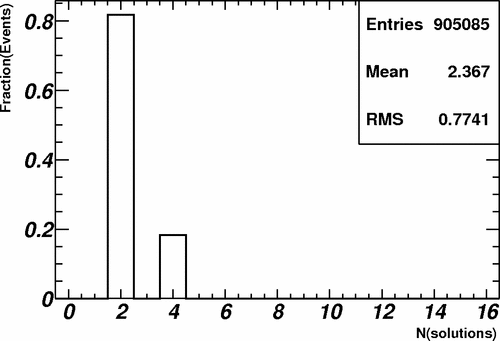
\includegraphics[width=0.6\textwidth]{05_kinReco/plots/medium.png}
  \caption{Number of solutions of the equation \ref{eq:eqLSf}. The distribution is normalized to one. The generated data used for this check
  is produced before any radiation. The figure is taken from \cite{LSpaper}.}
  \label{fig:LSNsol}
\end{figure}

Under the real conditions a sizable amount of the events will find no solutions of the kinematic equations (\ref{alg:LS1}--\ref{alg:LS6})
because of an imperfect reconstruction of the detector objects. But in the other cases there is a possibility to find up to four solutions.

\section{Solution Search}

There are several problems arising during the $t\bar{t}$ kinematics reconstruction. A trace to some of them was already given in the previous
section. Following challenges have to be dealt:

\begin{itemize}
 \item \textit{Measurement fluctuations}. As mentioned in section \ref{sec:MatBg}, there might be no solutions found for a certain combination
 of leptons, jets and missing transverse energy if some of them are inaccurately reconstructed and due to some measurement fluctuations the equation
 is lead to an unphysical region.
 %
 \item \textit{Multiple solutions of the kinematic equations}. As discussed in section \ref{sec:MatBg} the solution of the equation \ref{eq:eqLSf}
 provides up to four correct solutions while a real neutrino has only one momentum.
 %
 \item \textit{Multiple combinations of leptons and jets}. An event with a $t\bar{t}$ decaying to a dilepton final state has minimum two leptons and two
 jets. But there is no sign if a jet comes from $t$ or a $\bar{t}$. For this reason each jet is being paired to one of the leptons, and then to another
 to form a $t$ or $\bar{t}$ candidate. Thus an event with two leptons and two jets has two possible $t\bar{t}$ candidates. In case of multiple jets
 in the event, the number of $t\bar{t}$ will be $N!$, where $N$ is a jet multiplicity.
\end{itemize}

\subsection{Measurement fluctuations}

The challenge of rescuing the events which are lost due to the measurement fluctuations can be solved by varying the measured objects energies and
momentum directions. That would increase a chance of pushing the kinematics back to physical region. This idea was implemented by reconstructing
each event 100 times, each time shifting relevant observables randomly according to their resolution determined from the Monte Carlo.

The lepton and jet energies and momenta were smeared. The energy variation was performed through multiplication of an actual reconstructed energy value
by a correction factor $f(E) = \frac{E_{reaco}}{E_{true}}$. Here the $E_{reco}$ is the lepton or jet energy taken from the MC on the reconstructed level
and the $E_{true}$ is the true energy of the same object on the particle level. The distributions for the $f(E)$ which are used for random correction
factor choice are shown on the Figure \ref{fig:fE}. The shape of these distributions is energy independent (see Appendix !!!), thus they are obtained in
the complete kinematic region.

\begin{figure}[t]
\centering
\begin{subfigure}
  \centering
  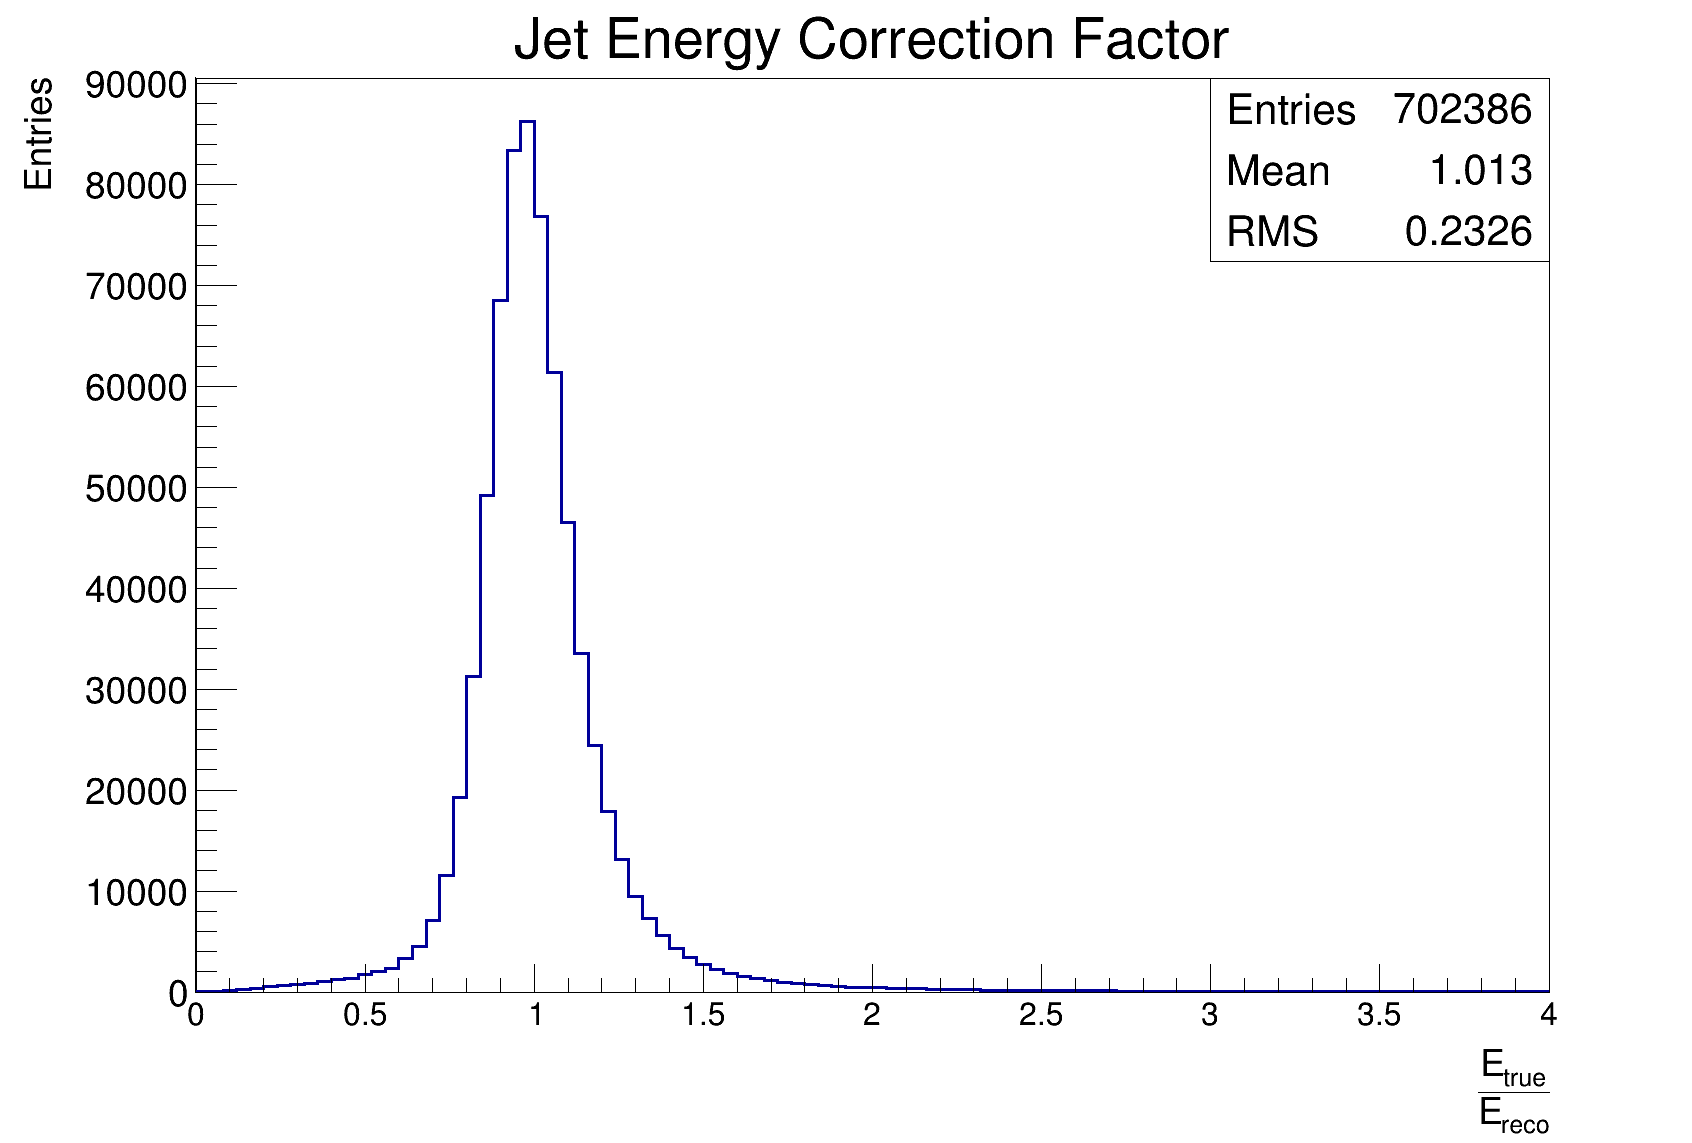
\includegraphics[width=0.48\textwidth]{05_kinReco/plots/fE_jet.png}
\end{subfigure}
\begin{subfigure}
  \centering
  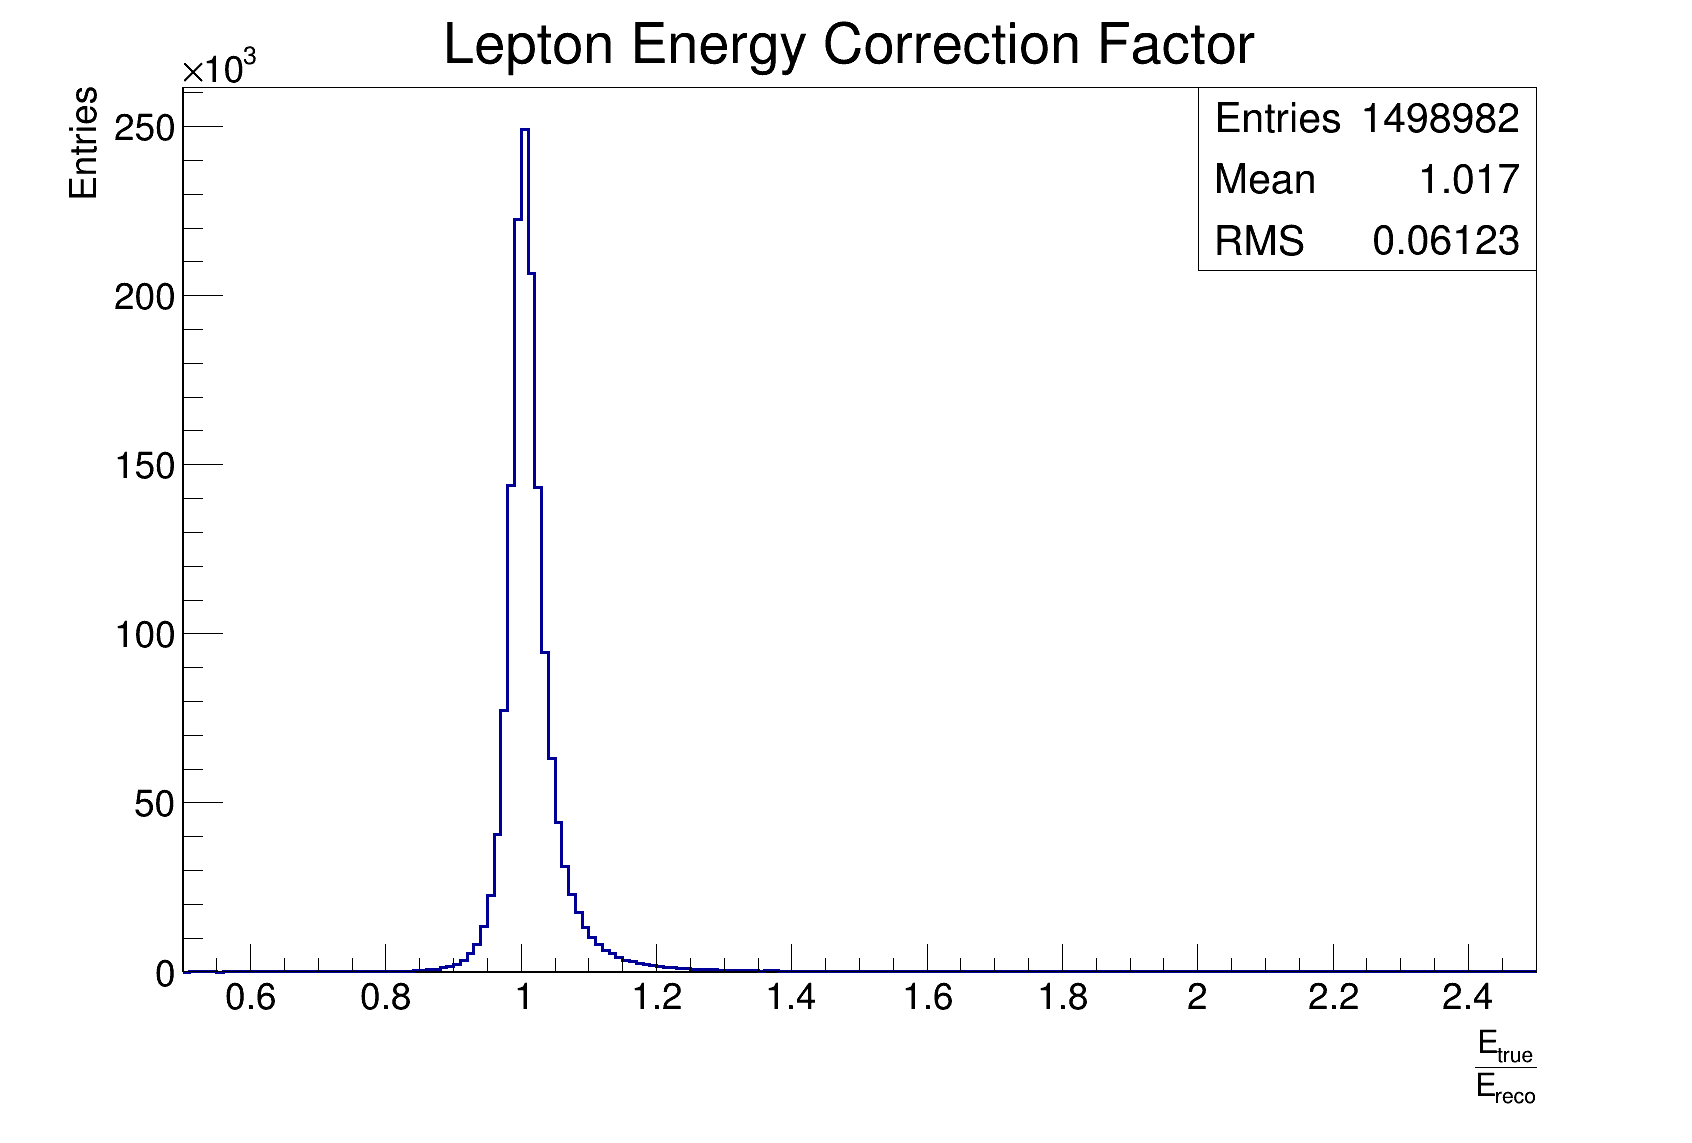
\includegraphics[width=0.48\textwidth]{05_kinReco/plots/fE_lep.png}
\end{subfigure}
\caption{Distributions of the energy correction factors used for the energy smearing in the kinematic
reconstruction of the top-quark kinematics. The factor distribution for jets is shown on the left and for
the leptons -- on the right.}
\label{fig:fE}
\end{figure}

Additionally to the energy variation a random gaussian smearing in a random diraction around the nominal direction is applied. The resolutions for
the gaussians are taken from the MC distributions presented on the Figure \ref{fig:dAngle}. These distributions are also independent of leptons and
jets kinematics (see Appendix !!!) and thus the resolution applied for smearing is averaged over the whole kinematic range.

\begin{figure}[t]
\centering
\begin{subfigure}
  \centering
  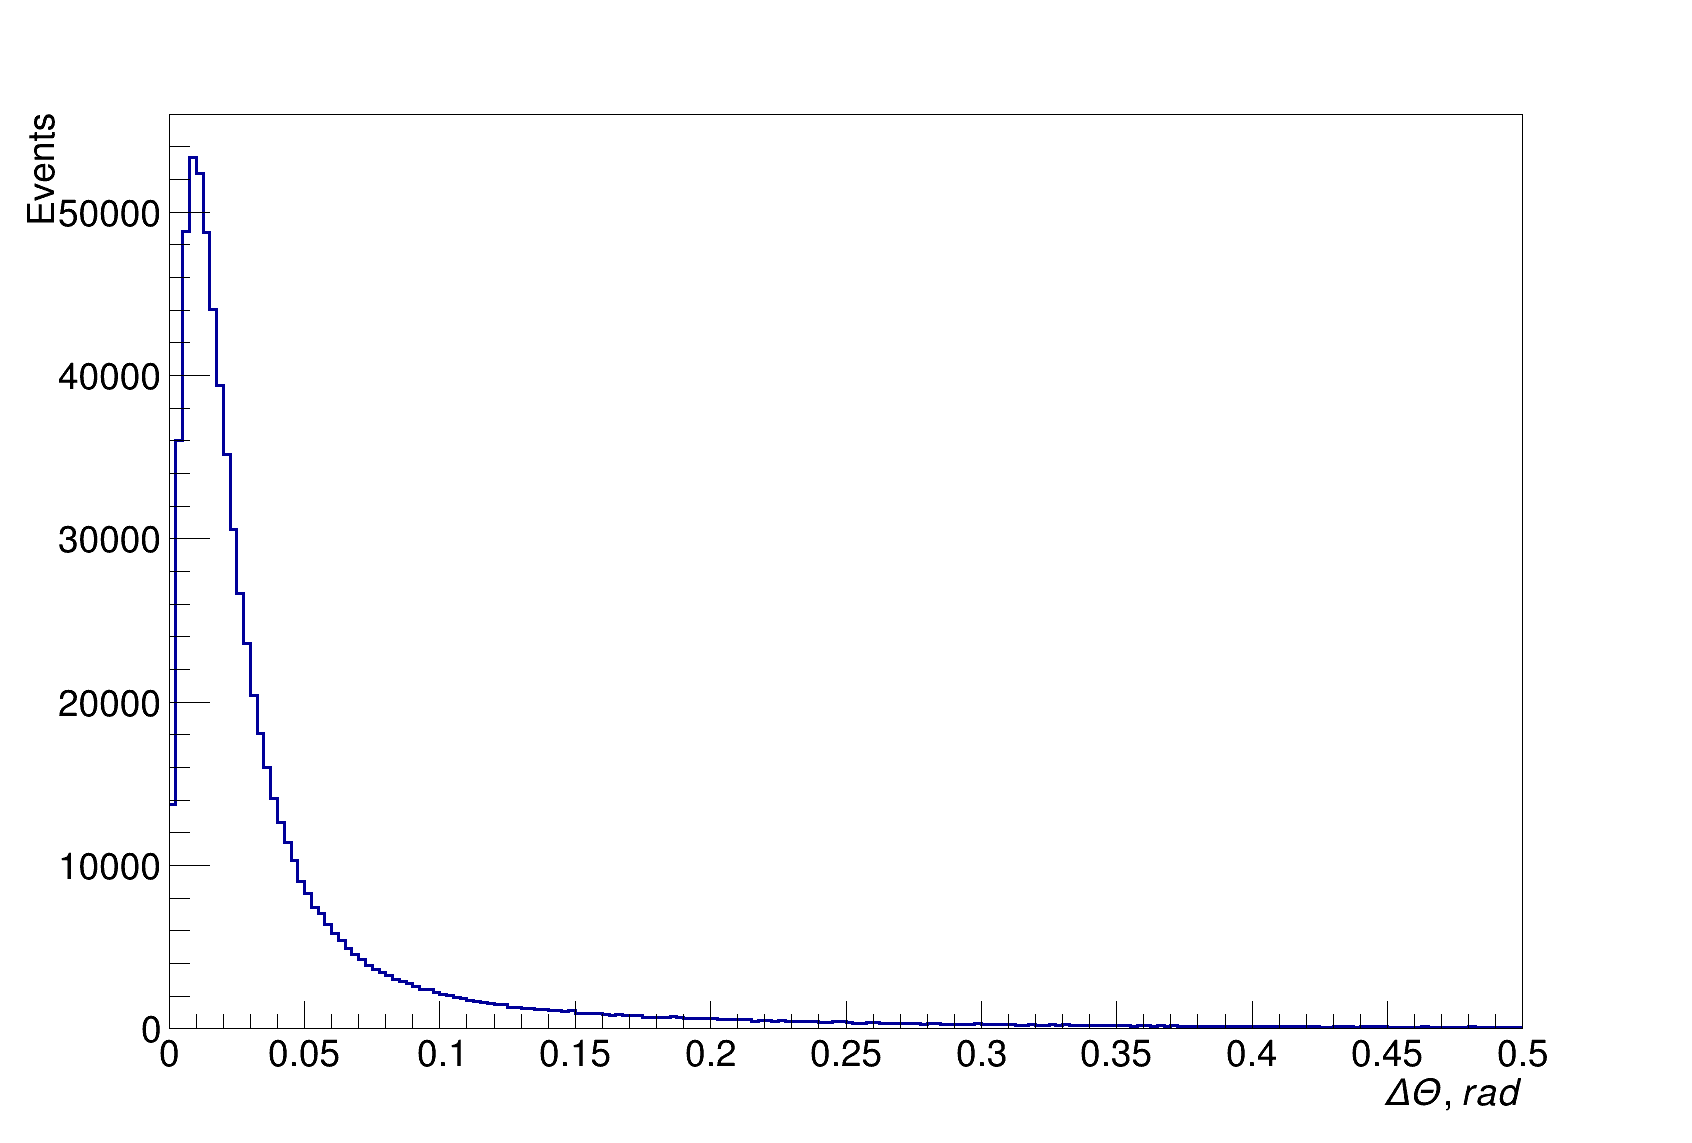
\includegraphics[width=0.48\textwidth]{05_kinReco/plots/dan_jet.png}
\end{subfigure}
\begin{subfigure}
  \centering
  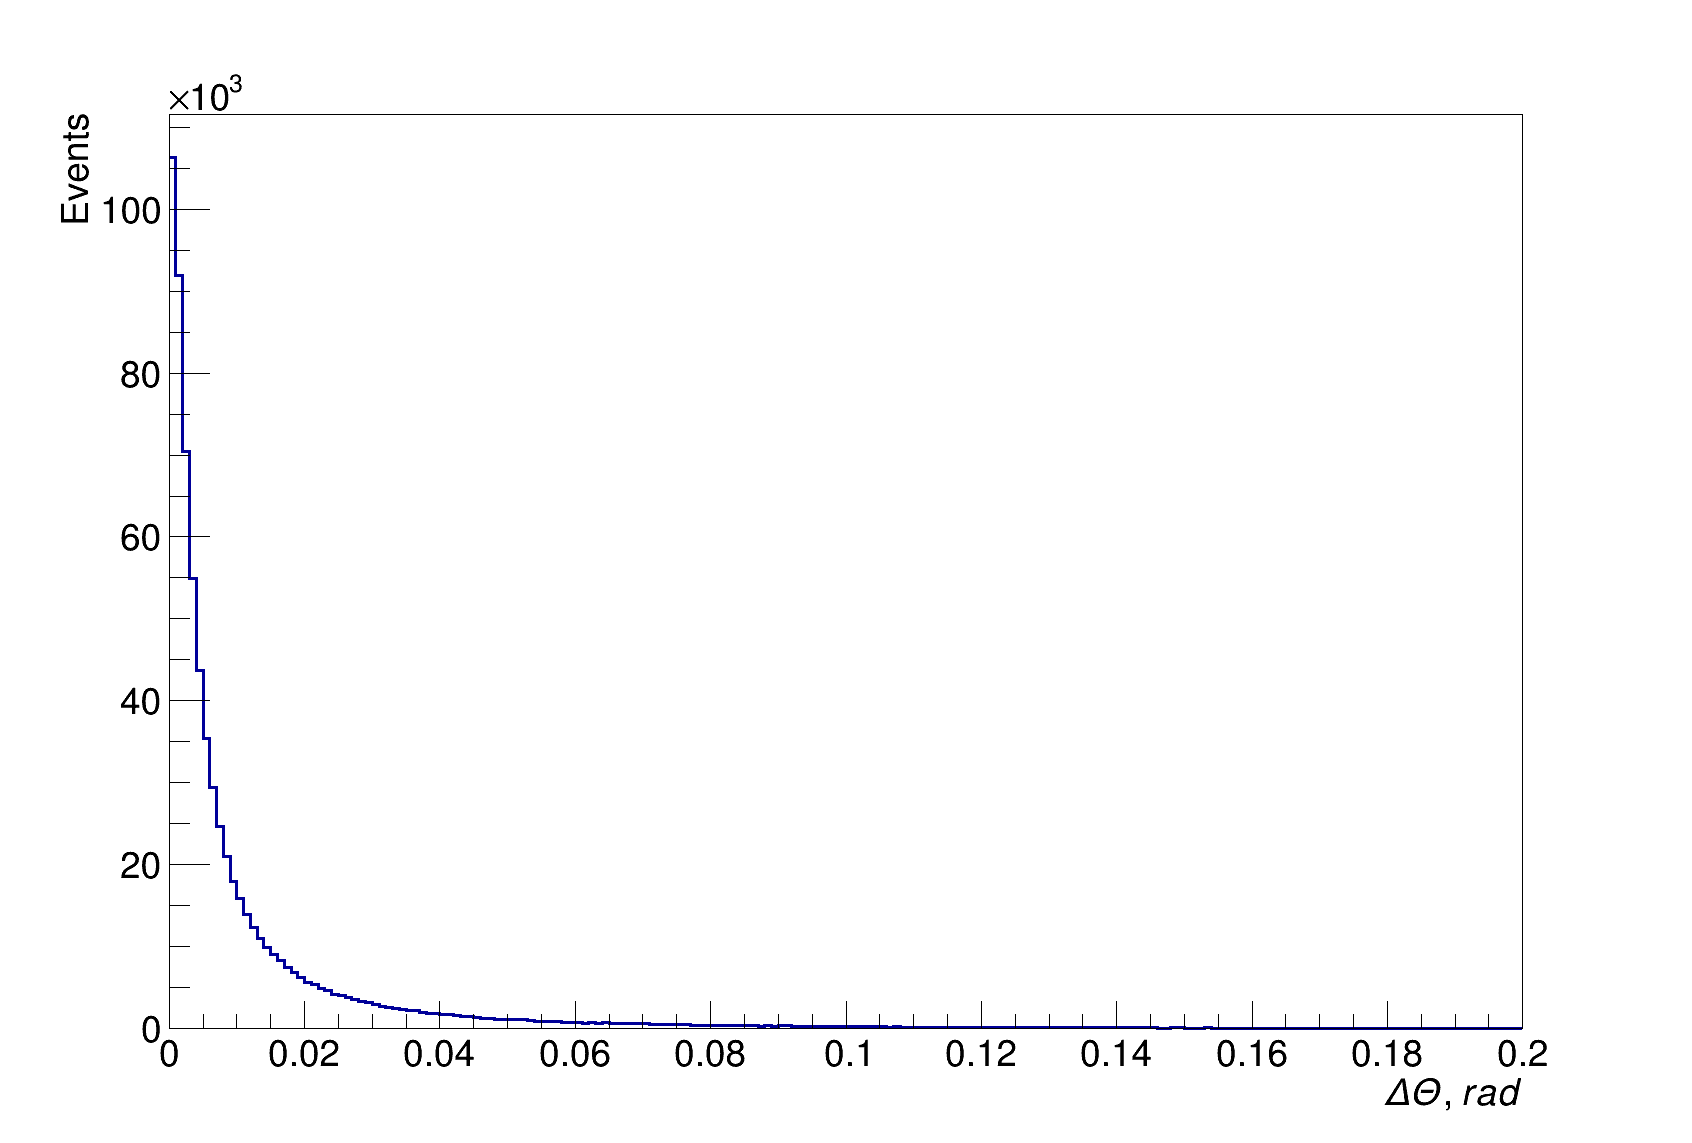
\includegraphics[width=0.48\textwidth]{05_kinReco/plots/dan_lep.png}
\end{subfigure}
\caption{Distributions of the angle between the particle level direction and the detector level direction.
The angle distribution for jets is shown on the left and for the leptons -- on the right.}
\label{fig:dAngle}
\end{figure}
% 
% \section{Performance}
% \subsection{Efficiency Studies}
% \subsection{Control Distributions}
% \subsection{Quality Studies}
